\documentclass[twoside,11pt]{article}

% Any additional packages needed should be included after jmlr2e.
% Note that jmlr2e.sty includes epsfig, amssymb, natbib and graphicx,
% and defines many common macros, such as 'proof' and 'example'.
%
% It also sets the bibliographystyle to plainnat; for more information on
% natbib citation styles, see the natbib documentation, a copy of which
% is archived at http://www.jmlr.org/format/natbib.pdf

\usepackage{jmlr2e}
%\usepackage{parskip}

% Definitions of handy macros can go here
\newcommand{\dataset}{{\cal D}}
\newcommand{\fracpartial}[2]{\frac{\partial #1}{\partial  #2}}
% Heading arguments are {volume}{year}{pages}{submitted}{published}{author-full-names}

% Short headings should be running head and authors last names
\ShortHeadings{95-845: MLHC Final Project}{LI}
\firstpageno{1}

\begin{document}

\title{Forecasting Postoperative Mortality after General Surgery Based on MIMIC III Data\\ Heinz 95-845: Machine Learning for Health Care}

\author{\name Xinmi Li \email xinmil@andrew.cmu.edu \\
       \addr Heinz College\\
       Carnegie Mellon University\\
       Pittsburgh, PA, United States
       } 

\maketitle

\begin{abstract}
  This study aims to use machine learning models to predict postoperative mortality for patients in intensive care units (ICU) after general surgery. Multiple machine learning algorithms are trained and tested with the data collected in Multiparameter Intelligent Monitoring in Intensive Care III (MIMIC III) database. Through these models, items considered to be significant in post-surgery care are examined and their contribution to post-surgery death are disccussed in this study. In this study, the performance of each algorithm is also compared with each other, to suggest on the most useful and reliable model that could be used in future postoperative mortality prediction.
\end{abstract}

\section{Introduction}
In medical field, the traditional method to analyzing the effect of an intervention is to conduct a randomized clinical trial and analyze the outcomes. Though high levels of recommendation could derive from them, with many limitations such as the size of population involved in the trial and ethical concerns, randomized clinical trials may not be able to be launched or completed, or the conclusions could be not broadly applicable. Besides, the complicated recruiting stage, the compliance issue of participants, and the long period of the trial and follow-ups make the randomized clinical trial unefficient and costly.

Recent advances in machine learning and the transfer from paper health records to eletronic health records have provided huge opportunities to health care research. With large volume of patient data and the high-speed data processing, we are now able to research on the topics that are used to be impposible for randomized clinical trial. 

MIMIC III database is a large and freely available database that consists of deidentified health-related data on over 40,000 patients collected from ICU of the Beth Israel Deaconess Medical Center between 2001 and 2012 \citet{cite1}. Some amount of progress on mortality prediction has been made by studying MIMIC III data. One research uses the abundance of ICU data to analyze the relationship between using selective serotonin reuptake inhibitors and the increase of mortality \citep{cite2}, but it only does statistical tests on the outcome instead of building machine learning models. And another reaserch makes mortality predictions among patients with sepsis and hypotension by using dynamic data during hypotensive episode\citep{cite3}. Although it only uses logistic regression to build the model, it has the movelty that using multiple perform measures to compare this model with traditional medical protocols. And another study builds a targeted real-time early warning score for septic shock by using lab data \citep{cite4}, which outperforms other widely-used protocols.

In this work, we use the MIMIC III data to predict the post-surgery mortality for ICU patients who just had genral surgery. Unlike to other studies using MIMIC data, this work makes the prediction not related to a specific condition. The purpose of it is to have a more general forecast that can be applied to all ICU patients with general surgery, and to provide a guide for nurses to provide better post-surgery care through the examination of indicators of mortality.

In Section 2, we provide background on the postoperative mortality. In section 3, we have a basic elaboration of the models used in this study. Then in section 4, experimental setup is provided to allow for replication of the study. Section 5 gives the results of the model. And more discussions on this study and related work are in section 6.

\section{Background} \label{background}
With more and more emphases on heath care quality and patient safety, lowering the postoperative risk is extremely significant. Although the national death rate from complications of medical and surgical care is decreasing over years \citet{cite5}, post-surgery death is still a big issue especially for the acute or unplanned surgery. Therefore, good postoperative care is important. To have a guidance on indicators of postoperative risk of death means not only better patient safety outcomes but also a relief from alert fatigue for nurses.

\begin{figure}[htbp]
  \centering 
  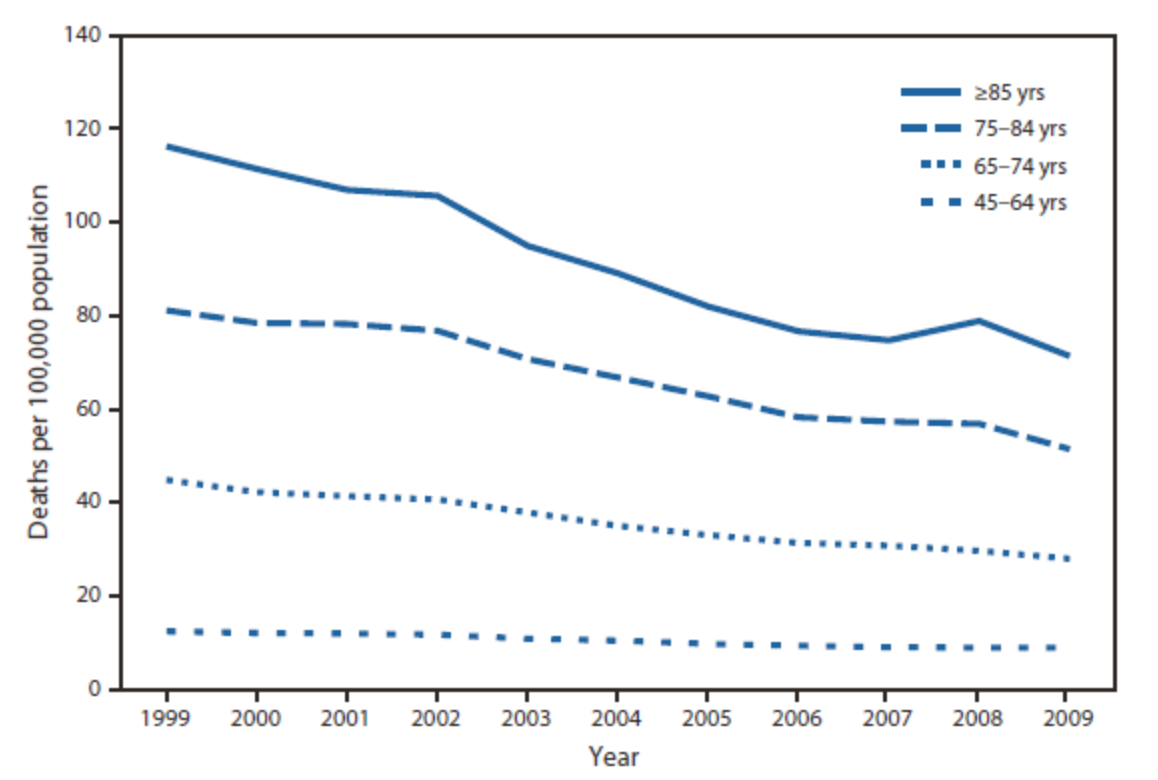
\includegraphics[height=8cm, width=12cm]{fig1} 
  \caption{Death Rate From Complications of Medical and Surgical Care Among Adults Aged ≥45 Years, by Age Group — United States, 1999~2009}
  \label{fig1} 
\end{figure} 

\section{Logistic Regression, Naive Bayes, Tree Augmented Naive Bayes, Decision Tree, and Random Forest Models} \label{model}
In this study, multiple machine learning models are used in R programming with packages: Logistic Regression, Naive Bayes, Tree Augmented Naive Bayes, Decision Tree, and Random Forest.

After training and testing all models, they are evaluated based on the accuracy of classification the outcome, receiver operating characteristic curve (ROC curve), and precision-recall curve (PR curve).

\begin{figure}[htbp]
  \centering 
  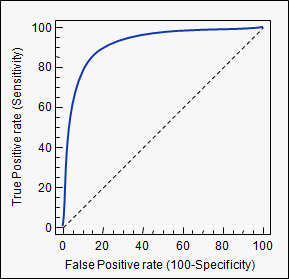
\includegraphics[height=7cm, width=7cm]{fig2} 
  \caption{ROC Curve; source: https://www.medcalc.org/manual/roc-curves.php}
  \label{fig2} 
\end{figure} 

\begin{figure}[htbp]
  \centering 
  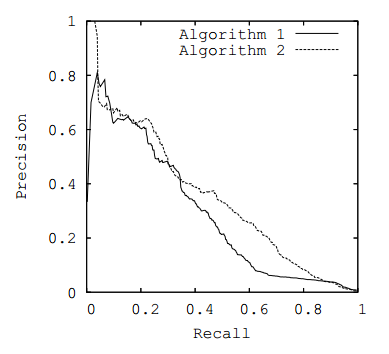
\includegraphics[height=7cm, width=7cm]{fig3} 
  \caption{PR Curve; source: https://www.quora.com/What-is-Precision-Recall-PR-curve}
  \label{fig3} 
\end{figure} 

\[Accuracy = \frac{True Positive + True Negative}{True Positive + False Positive + True Negative +False Negative}\]

\[Precision = \frac{True Positive}{True Positive + False Positive}\]

\[Recall = \frac{True Positive}{True Positive + False Negative}\]

Code is available at \url{https://github.com/xml93/MLforHC_FinalProject}.

\section{Experimental Setup} \label{experiment}

\subsection{Cohort Selection} 
The MIMIC III database contains over 40,000 patients' records and related health information. Since this study focuses on the patients who have general surgery and stay in ICU at the time of recording, only patients who have "ICU" as the cost center and "SURG" (which represents general surgery, other specific categories of surgery are marked respectively) as the current service. After selection, only 3580 patients are left. 

\begin{table}[htbp]
  \centering 
  \begin{tabular}{|c|c|c|c|c|c|c|} 
    Gender & Outcome (\%) & RR & O2 Saturation(\%) & Temp(F) & Systolic BP & HR\\ 
    \hline \\[-11pt]
    Female & Survival: 954 (61.5\%) & 18.72 & 89.07 & 98.33 & 115.81 & 87.81\\ 
    1551 & Death: 597 (38.5\%) & 19.56 & 90.93 & 97.86 & 116.80 & 87.95\\ 
    Male & Survival: 1164 (57.4\%) & 18.31 & 88.92 & 98.50 & 116.80 & 87.95\\
    2029 & Death: 865 (42.6\%) & 19.59 & 91.69 & 98.11 & 107.46 & 88.06\\ \hline 
  \end{tabular}
\end{table}

\subsection{Data Extraction} 
All datasets are downloaded from MIMIC III database and are in different spreadsheets of topics. Basic sql queries are used to link them. Since each patient has multiple admission records and each is related to general surgery, in order to predict the mortality after surgery, only the most recent admission is kept. And all other patient information is only kept for this most recent admission record. Each patient's admission has an ICD-9 Diagnosis code indicating the diagnosis. They are transformed into 19 groups using the first 3 digitd of ICD-9 code based on the ICD-9 diagnositic groups, making such data more informative.

\begin{figure}[htbp]
  \centering 
  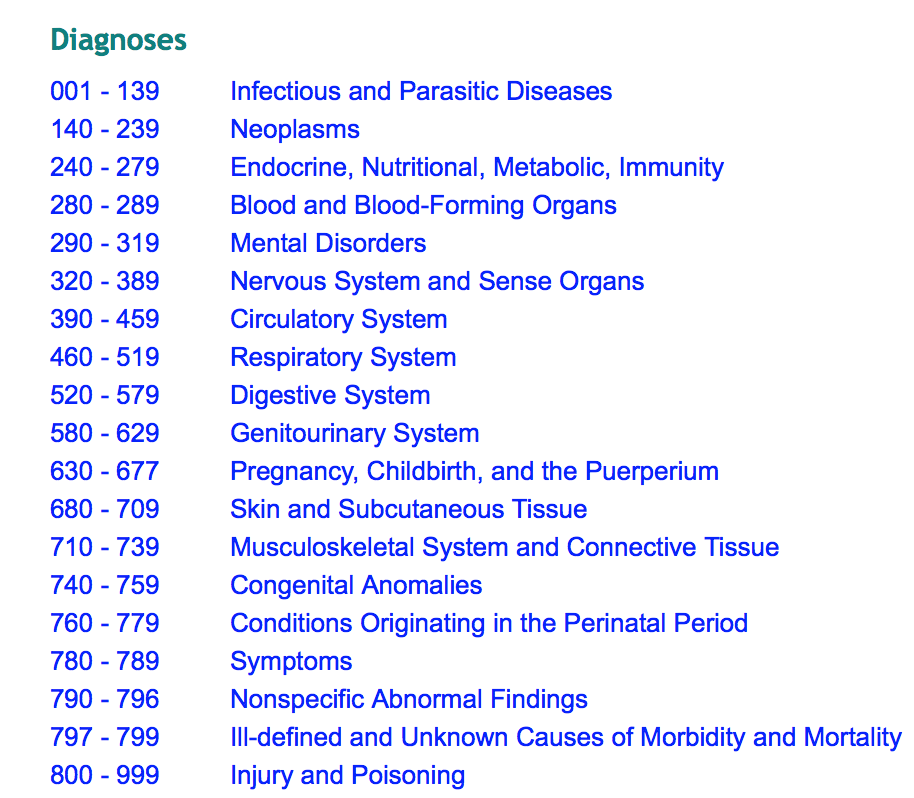
\includegraphics[height=8cm, width=8cm]{fig4}
  \caption{ICD-9 Diagnosis Group}
  \label{fig4} 
\end{figure} 

\subsection{Feature Choices} 
Features used in the model are mainly based on protocols used in the postoperative care. We want to know which medication and what physiology of patient are useful indicators of post-surgery death. Therefore, top 10 medications with highest prescription frequency are selected. They are Lactated Ringers ("LR1000"), Insulin ("INSULIN"), Furosemide ("FURO40I"), Magnesium Sulfate ("MAG2PM"), Sodium Chloride 0.9\% Flush ("NACLFLUSH"), Metoprolol ("METO5I"), Depakote 500 mg ("NS500"), 250 cc of 5 \% dextrose solution ("D5W250"), Depakote 250 mg ("NS250"), and Depakote 1000 mg ("NS1000"). And the medications are trandsormed into a set of vectors with binary value indicating whether each patient has had such drug. And the patient's physiologies that matter in postoperative care are: respiratory rate ("RR"), oxygen saturation ("SPO2"), temperature ("T"), systolic blood pressure ("BP"), pulse rate, and level of consciousness, according to the National Early Warning Score (NEWS Score) \citet{cite6}. Due to the few record size of pulse rate and the difficulty to categorize consciousness level from the raw data, the last two physiologies are not included in this study. The other 4 physiologies have abundant data in the chartevent table, which means they are recoreded several times within each admission. The mean value of each physiology is calculated as the feature value. 

After checking the missing pattern of each colomn, colomns with over 50\% missing values and patients with over 5 missing items are dropped. And the remaining missing values are all the averaged physiologies in the previous feature selection step instead of direct records in raw data, so they are missing at random. R package "amelia" is used to impute the missing value for the remaining dataset, with 5 folds. However, after imputation, there are still 61 patients with less than 2 missing values unable to be imputed, so they are dropped.

\subsection{Evaluation Criteria and Method Comparison}
Since the existing models used to predict the mortality each focuses on a specific disease or condition and the models built in this study are more general and relatively novel in providing general guidance for postoperative care, models in this study are not compared to existing models. Instead, the models themselves are compared against each other to evaluate the performance, by using accuracy, ROC curve, and PR curve.

\section{Results} \label{results}
The variable importance for each algorithm is showed repectively in each subsection, except for Naive Bayes and Tree Augmented Naive Bayes (no method to show the variable importance), to find the useful indicators of postoperative mortality. And the performance of each algorithm is evaluated and compared to decide on the best model.

\subsection{Results on Logistic Regression} 
After 2 rounds of training the Logistic Regression model, the final model has the features and importance as plotted below.

\begin{figure}[htbp]
  \centering 
  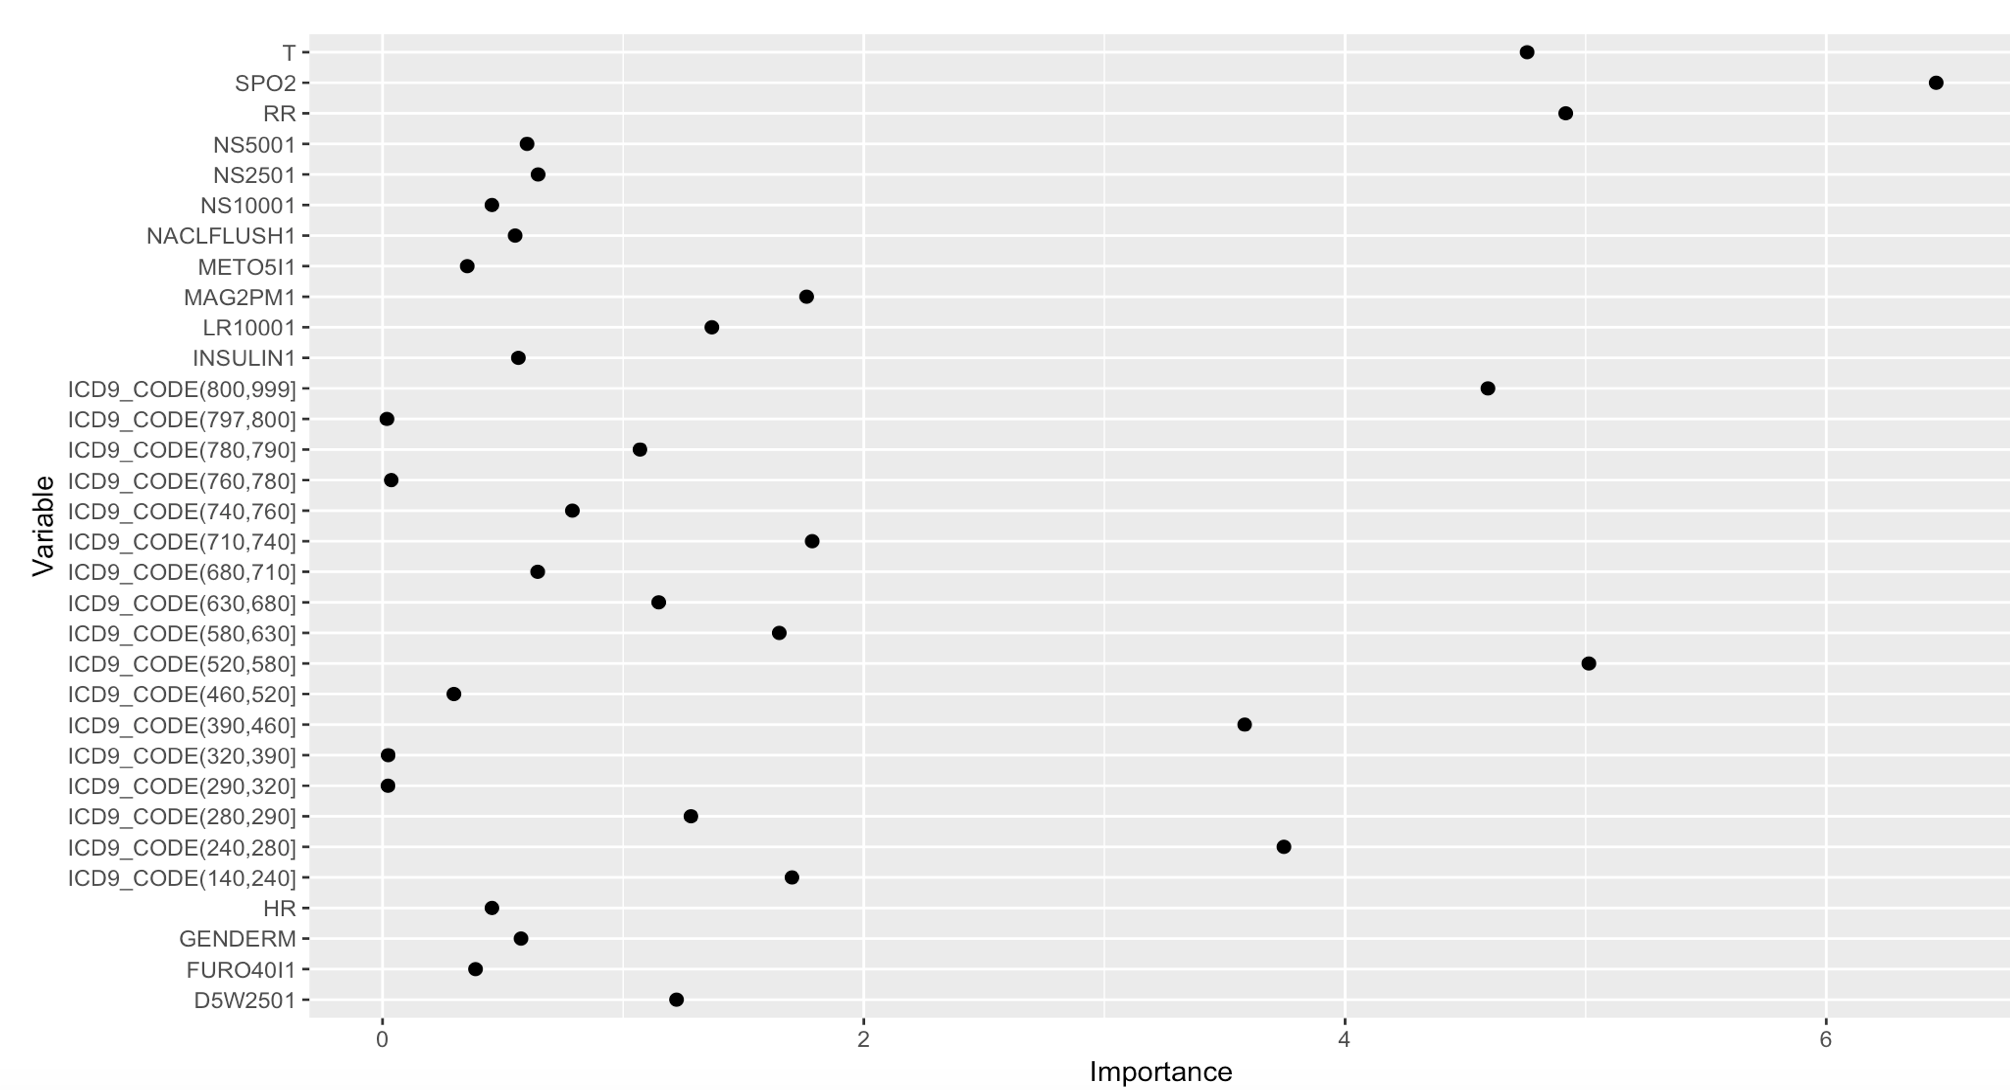
\includegraphics[height=7cm, width=14cm]{fig5} 
  \caption{The variable importance in predicting mortality of Logistic Regression}
  \label{fig5} 
\end{figure} 

From the plot we can know that the importance of all variables in this model is not very high, which means that they are not very useful in predicting the outcome. How these variables contribute to the postoperative mortality are listed below.

\begin{table}[htbp]
  \centering 
  \begin{tabular}{|c|c|c|} 
     Coef & Estimate & p-value\\ 
    \hline \\[-11pt]
    Intercept & 19.608118 & 0.000711\\ 
    Endocrine, Nutritional, Metabolic, Immunity & -1.664949 & 0.000167\\ 
    Circulatory System & -0.996860 & 0.000165\\
    Digestive System & -1.023103 & 0.00000026\\
    RR & 0.084609 & 0.0000004\\ 
    SPO2 & 0.079917 & 0\\
    T & -0.285080 & 0.000002\\ \hline 
  \end{tabular}
\end{table}

Based on this model, features of the patient's respiratory rate, oxygen saturation, temperature, and whether the patient's diagnosis is related to Endocrine, Nutritional, Metabolic, Immunity / Circulatory System / Digestive System are of significance in predicting post-surgery death.

\subsection{Results on Desicion Tree} 
The Decision Tree after pruning is shown below.

\begin{figure}[htbp]
  \centering 
  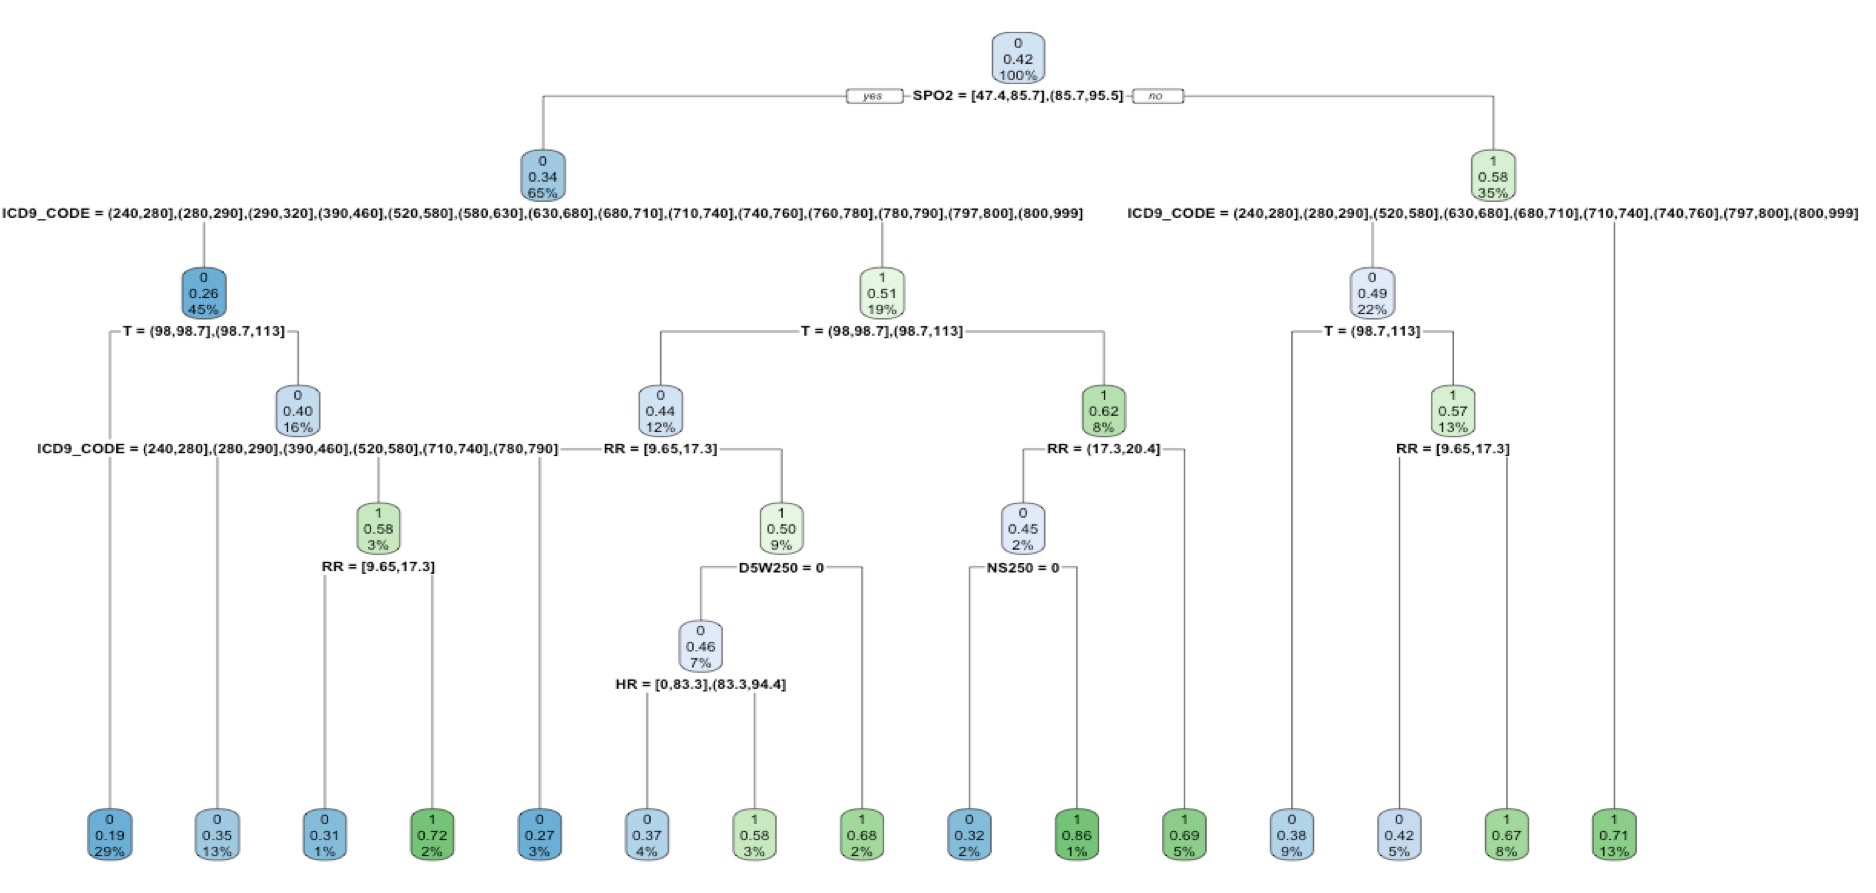
\includegraphics[height=7cm, width=14cm]{fig6} 
  \caption{Decision Tree}
  \label{fig6} 
\end{figure} 

\begin{figure}[htbp]
  \centering 
  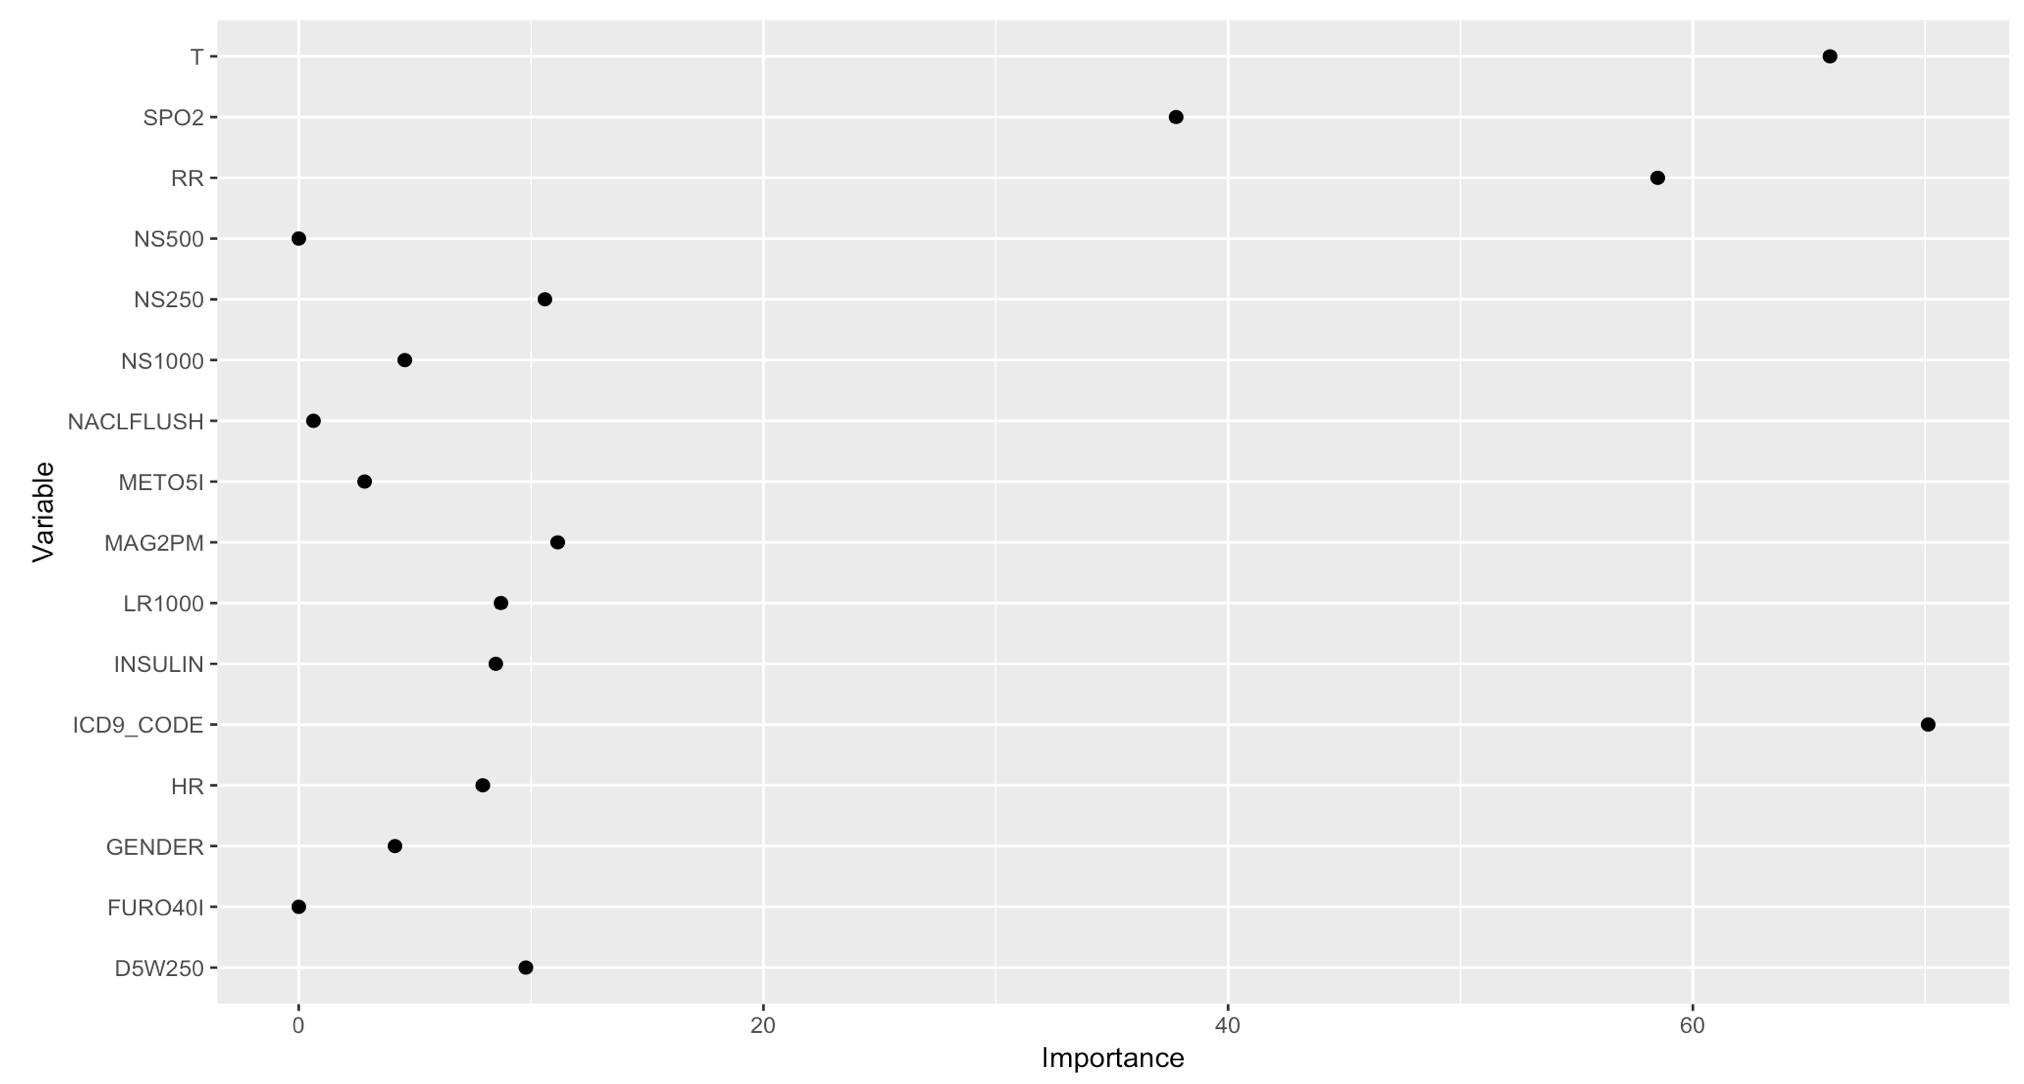
\includegraphics[height=7cm, width=14cm]{fig7} 
  \caption{The variable importance in predicting mortality of Decision Tree}
  \label{fig7} 
\end{figure} 

Here we can find that ICD-9 code (diagnosis group) and the patient's respiratory rate and oxygen saturation have a really high contribution to the patient's mortality. Also, some medications such as Magnesium Sulfate and Depakote are also strong indicators.

\subsection{Results on Random Forest}

\begin{figure}[htbp]
  \centering 
  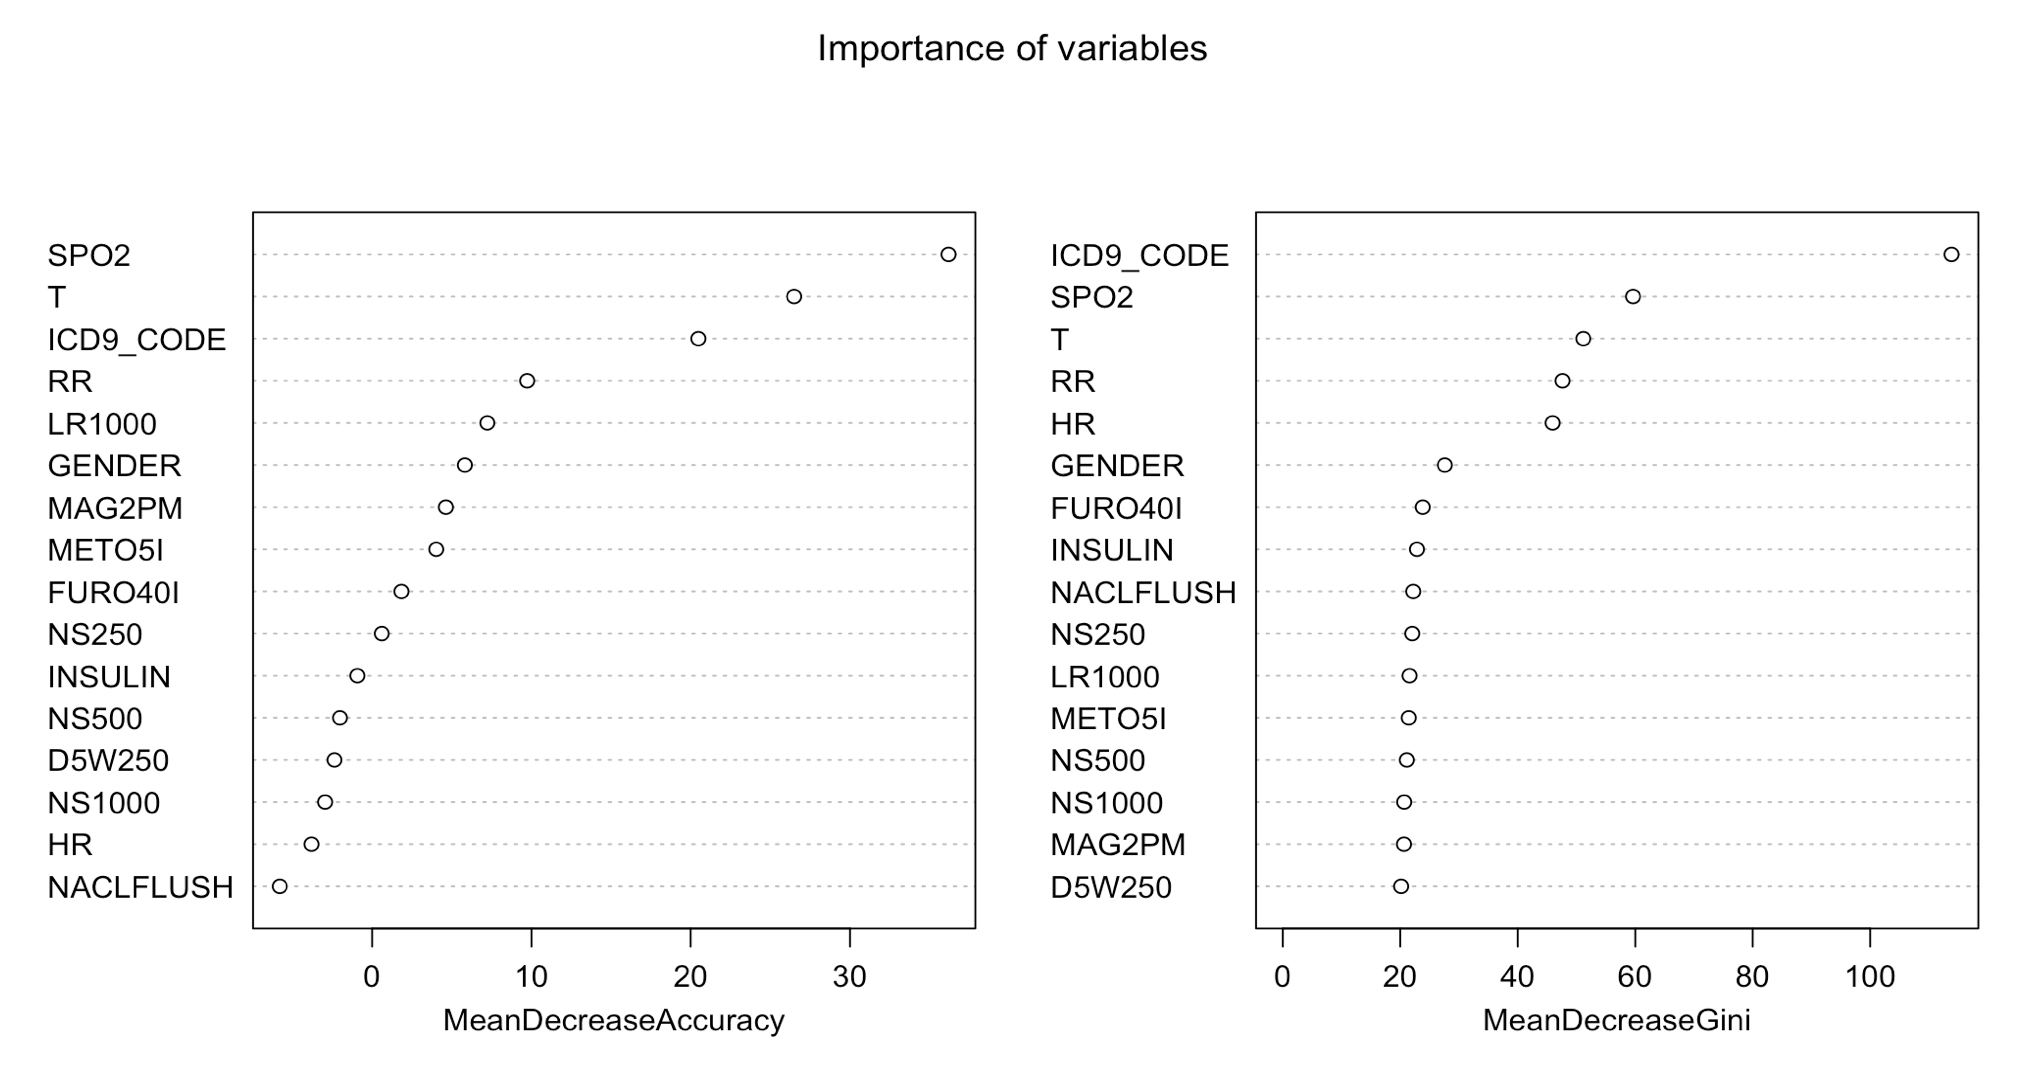
\includegraphics[height=7cm, width=14cm]{fig8} 
  \caption{The variable importance in predicting mortality of Random Forest}
  \label{fig8} 
\end{figure}

Here Random Forest uses 1000 as the number of trees and have votes on all trees to decide the contribution of each variable to the outcome. We can find that diagnosis, patient's temperature, oxygen saturation, and respiratory rate are still the top 4 variables that contribute the most to postoperative mortality, both on accuracy and Gini. Other features are not so significant or have inconsistent contribution regarding the model accuracy and Gini.

\subsection{Model Evaluation and Comparison}
\begin{table}[htbp]
  \centering 
  \begin{tabular}{|c|c|c|} 
     Method & Accuracy & 95\% Confidence Interval\\ 
    \hline \\[-11pt]
    Logistic Regression & 0.6473 & 0.6215~0.6732\\ 
    Naive Bayes & 0.6588 & 0.6331~0.6845\\ 
    Tree Augmented Naive Bayes & 0.6321 & 0.6059~0.6582\\
    Decision Tree & 0.6580 & 0.6323~0.6837\\
    Random Forest & 0.6351 & 0.6090~0.6612\\ \hline 
  \end{tabular}
\end{table}

\begin{figure}[htbp]
  \centering 
  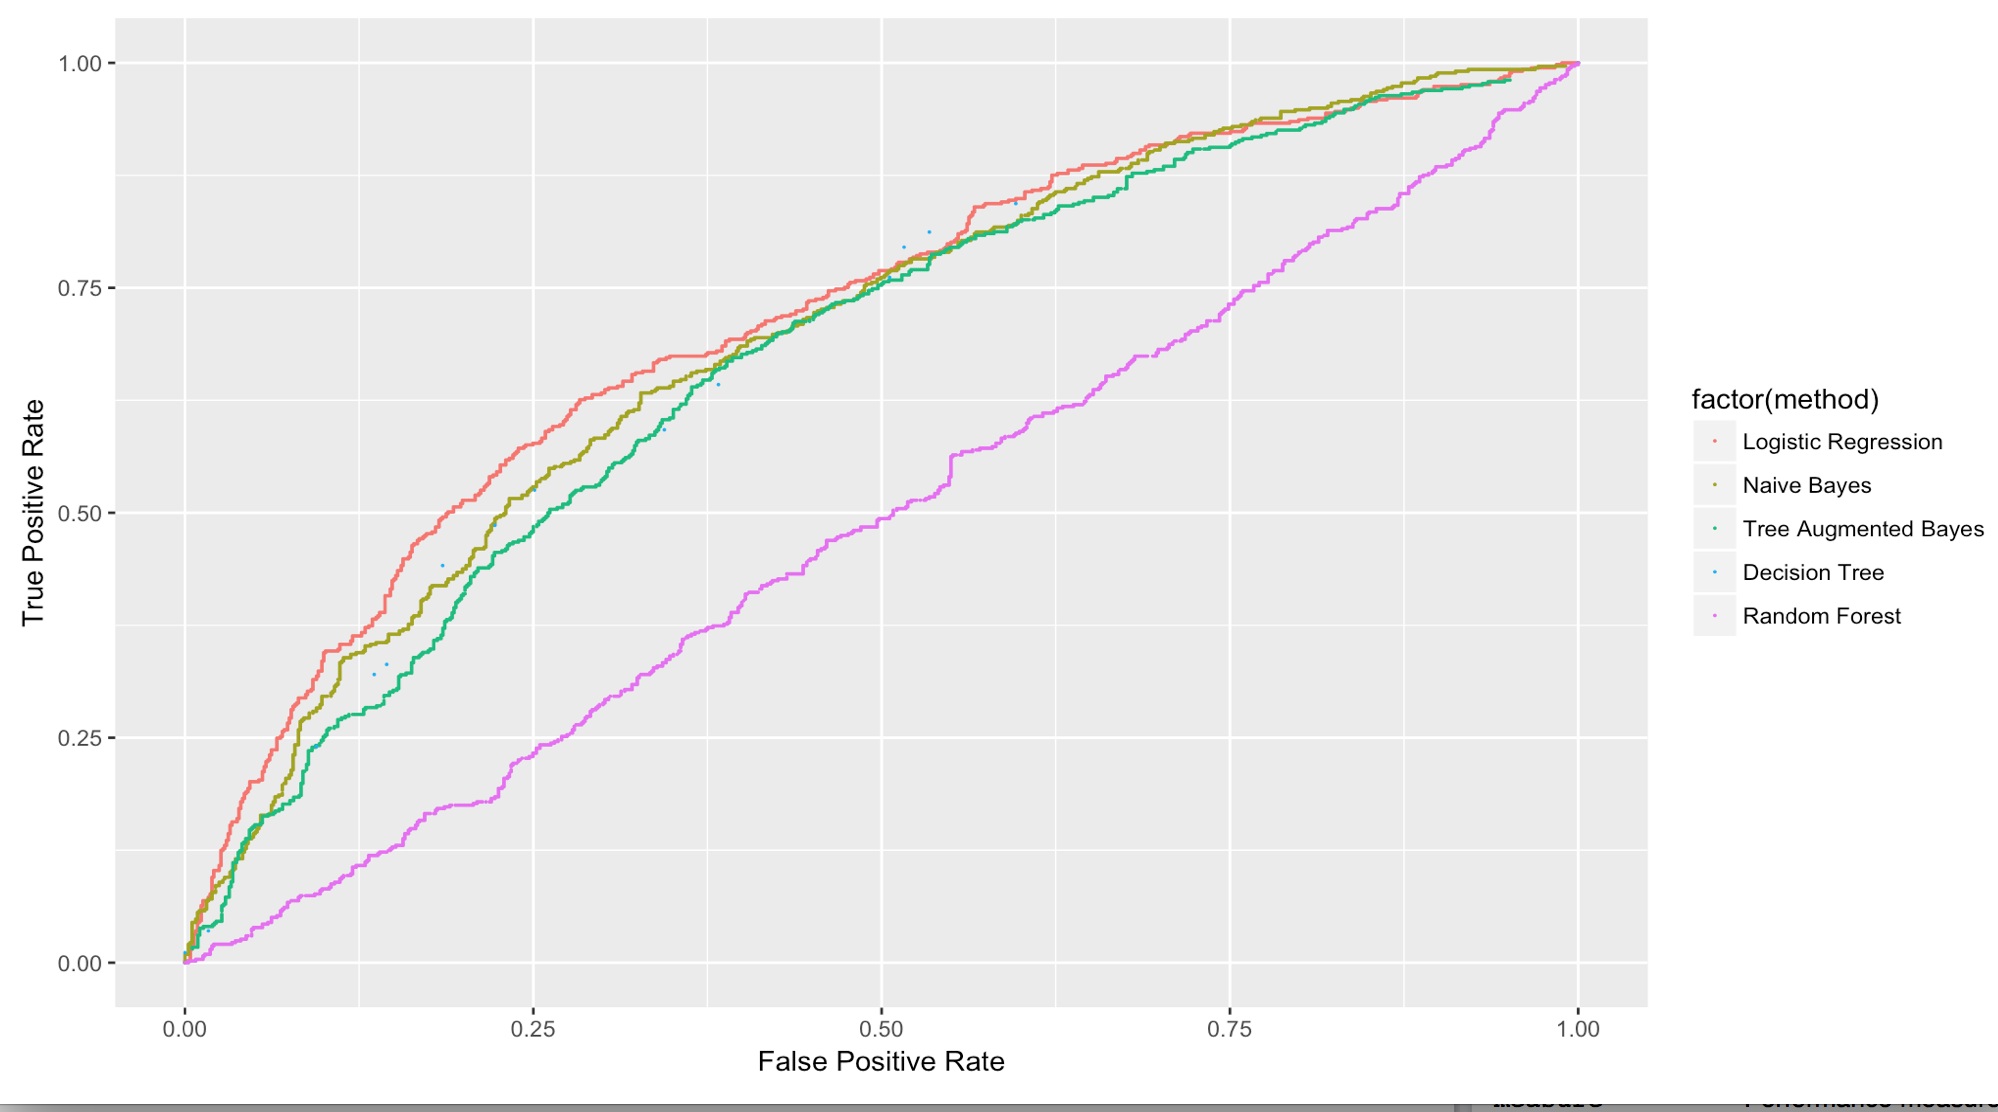
\includegraphics[height=8cm, width=15cm]{fig9} 
  \caption{ROC Curve}
  \label{fig9} 
\end{figure}

\begin{figure}[htbp]
  \centering 
  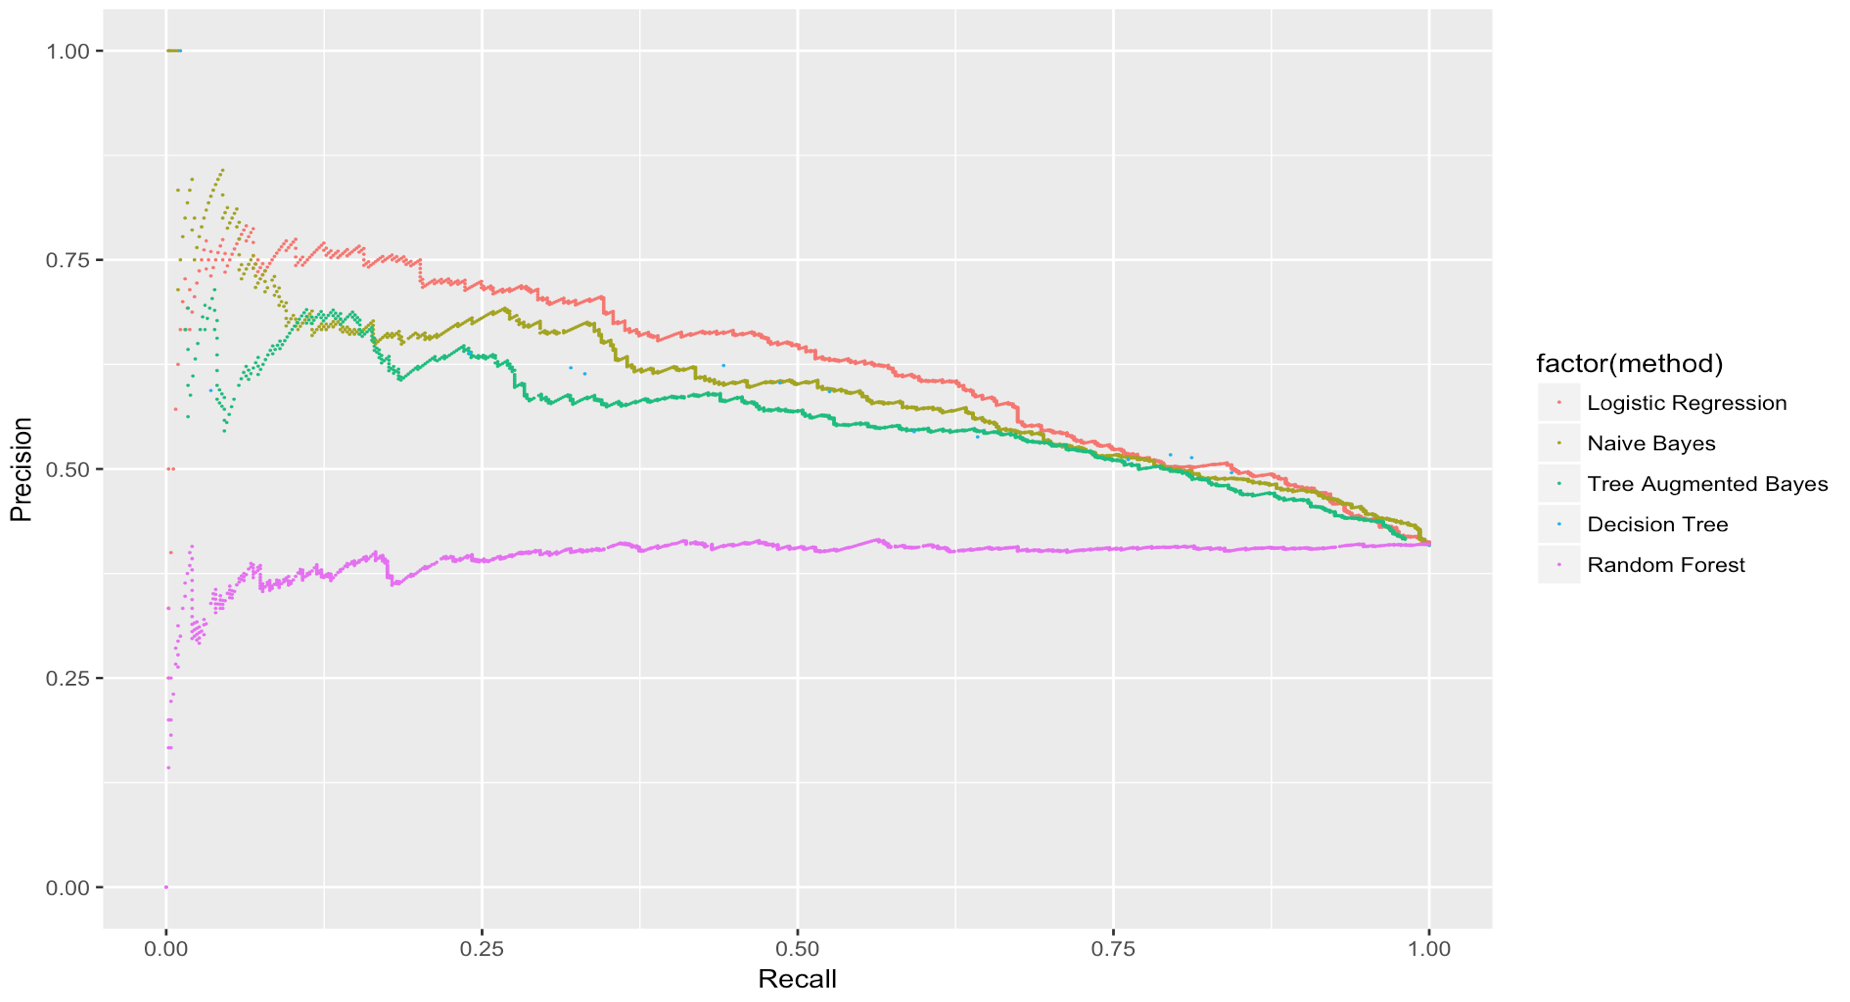
\includegraphics[height=8cm, width=15cm]{fig10} 
  \caption{PR Curve}
  \label{fig10} 
\end{figure}

Based on accuracy, Naive Bayes and Decision Tree outperform other models since they have a higher accuracy and also confidence interval. However, when looking at the ROC and PR curves, Logistic Reggression has the curve dominates other algorithms. Logistic Regression also has a relatively high accuracy. Combining the three measures, Logistic Regression is an effective model to predict post-surgery death and the features selected in this model are useful indicators.

\section{Discussion and Related Work} 



\section{Conclusion} 
Summarize your work one more time, this time assuming the reader has read your paper.
Build suspense for what your next extension to this method would be.

% ACKNOWLEDGEMENTS ONLY GO IN THE CAMERA-READY, NOT THE SUBMISSION
% \acks{Many thanks to all collaborators and funders!}

\bibliography{citation}

\appendix
\section*{Appendix A.}
Some more details about those methods, so we can actually reproduce them.

\end{document}
